\section{Lezione del 16 novembre}
SAT è stato il primo problema identificato come NP-complete ed è stato usato per riconoscere gli altri problemi NP-complete.\\ La descrizione di una NDTM deve quindi corrispondere ad una $\phi$ di SAT per far vedere che tutti i problemi NP si riducono a SAT. Ci basta far vedere che $SAT<_T \Pi$ per far vedere che $\Pi$ è NP-complete. Se dimostriamo che $SAT$ si riduce a $\Pi$, se ci si presenta un secondo problema, se dimostriamo che questo si riduce a $\Pi$ o SAT dimostro che anche il secondo problema è NP-complete. \\ 

Si ha che il problema del ciclo hamiltoniano e TSP, decisionali, siano NP-complete.\\ 

Vediamo che $SAT<_T 3SAT$, $3SAT$ è una soddisfacibilità che ha tre letterali in ogni clausola. Ho in input una formula $\phi$ che deve diventare una $\phi_3$ tale che $\phi$ è soddisfacibile sse $\phi_3$ lo è. 
La formula $\phi$ ha tante clausole in congiunzione tra loro con un numero arbitrario di letterali ma $\phi_3$ deve averne altrettante ma con soli tre letterali per clausola. \\
Numero di clausole presenti: 
\begin{enumerate}
    \item Qualora si abbiano clausole in $\phi$ con un solo letterale si aggiungono due letterali (che indichiamo con $z$) in modo però che la veridicità sia basata solo sulla variabile iniziale (questo vale per tutte le trasformazioni che stiamo per mostrare, ovvero la veridicità deve valere in base solo alle variabili iniziali della formula $\phi$). La clausola che conteneva solo un letterale, che chiamiamo $x_1$, per assicurare la veridicità, ha bisogno di essere espressa nel modo: $(x_1\lor z_1\lor z_2)\land (x_1\lor \overline{ z_1}\lor z_2)\land (x_1\lor z_1\lor\overline{ z_2})\land(x_1\lor\overline{ z_1}\lor\overline{ z_2})$
    \item Se invece avessi una formula con due letterali quello che serve è aggiungere una sola variabile, ritrovandoci quindi: $(x_1\lor x_2\lor z_1)\land (x_1\lor x_2\lor \overline{ z_1})$
    \item Una formula a tre letterali resta ovviamente invariata.
    \item Quelle a più letterali vanno spezzate (aggiungendo poi variabili). Per esempio, avendo quattro letterali, otterrei: $(x_1\lor x_2\lor z_1)\land (\overline{ z_1}\lor x_3\lor z_2)\land (\overline{ z_2}\lor x_4\lor z_3)\land\cdots\land(z_{n-3}\lor x_{n-1}\lor x_n)$
\end{enumerate}
Si vede che ogni formula di SAT può essere trasformata in una di 3SAT e quindi anche quest'ultimo è NP-complete. Si dimostra che invece 2SAT non è NP-complete ma ogni $K$SAT, con $K>2$, è NP-complete.\\ 

Torniamo a parlare di TSP, non di decisione. Ho capito che serve tempo esponenziale per risolverlo quindi si può pensare che sia NP-complete. 
Passo quindi alla versione di decisione. Vedo però che ciclo hamiltoniano, che è NP-complete, si riduce a TSP decisionale. Questo ci dice che è anch'esso NP-complete. Abbiamo comunque che TSP è più difficile del suo problema decisionale, infatti D-TSP si riduce a TSP. Si ha quindi che TSP è \textbf{NP-hard}, ovvero il problema problema stesso non è in NP e tutti i problemi NP si riducono ad esso. Non essendo un problema di decisione, quindi non avendo un linguaggio associato, risulta che TSP non è in NP.

\subsection{Rapporto spazio e tempo}
Definisco la \textbf{funzione di complessità spaziale} come: $f:\mathbb{N} \to \mathbb{N}$ con $f(n)$ che è il massimo numero di caselle utilizzate da una TM per decidere un certo linguaggio $L$, analizzando tutte le istanze di una certa dimensione $n$ con $n=|x|$. Sappiamo che, dal punto di vista del tempo: $ P= \displaystyle \bigcup_{k\geq 1}dtime(n^k)$ e $ NP=\displaystyle  \bigcup_{k\geq 1}ntime(n^k)$

Definiamo la \textbf{classe DSPACE} come, lo spazio non deterministico, ovvero l'insieme di tutti i linguaggi tali che sono decisi da una TM in spazio $\mathcal{O}(f(n))$. Si ha che lo spazio corrisponde a $PSPACE=\displaystyle \bigcup_{k\geq 1}DSPACE(n^k)$ avendo quindi limite polinomiale.\\
 
Analogamente definiamo la \textbf{classe NSPACE} come l'insieme di tutti i linguaggi tali che sono decisi da una NDTM in spazio $\mathcal{O}(f(n))$. Si ha che lo spazio è $NPSPACE=\displaystyle \bigcup_{k\geq 1}NSPACE(n^k)$ avendo quindi limite polinomiale.\\

Come vale: $P\subseteq NP$n vale anche: $PSPACE\subseteq NPSPACE$ e per dimostrarlo mi concentro su una macchina che si preoccupa solo dello spazio
e non del tempo.\\

Prendiamo nuovamente il problema SAT e quindi ragioniamo sulla NDTM. Vediamo che SAT è in NPSPACE infatti capisco che ramo scegliere e tale ramo ha una casella per letterale, avendo spazio $n$. Vediamo se appartiene anche a PSPACE. \\

Una DTM potrebbe provare tutte le possibilità in tempo esponenziale ma in spazio polinomiale in quanto si sovrascrivono ad ogni tentativo le varie caselle indicanti gli assegnamenti di verità ma la cardinalità di tali caselle è sempre la stessa, una per ogni letterale, ovvero $n$. Quindi ho che $SAT\in PSPACE$ anche se non è un'informazione così eclatante a causa del tempo esponenziale.

\begin{teorema}{Teorema di Savitch}{}
  Si dimostra che:  $PSPACE=NSPACE$\\
  Quindi la DTM e la NDTM hanno la stessa potenza dal punto di vista dello spazio di calcolo.
\end{teorema}

La dimostrazione si basa sull'idea di \textbf{raggiungibilità di configurazione}. Quindi un problema è definibile all'interno delle TM come \textbf{configurazione raggiungibile}. Questo corrisponde al capire se una macchina può andare da una certa configurazione iniziale $c_i$ ad una finale $c_f$ in un certo numero di passi $t$, questo lo indichiamo come $(c_i,c_f,t)$. Una possibilità per capirlo sarebbe prendere una configurazione casuale $c_m$, che è una configurazione che si trova  a metà. Dico quindi che la macchina può fare $(c_i,c_f,t)$, se la macchina può fare anche: $\displaystyle \left(c_i,c_m,\frac{t}{2}\right)\land \displaystyle \left(c_m,c_f,\frac{t}{2}\right)$.\\
Con la stessa tecnica usata per creare le due configurazioni precedenti, procediamo nel suddividere, sempre attraverso Divide\&Impera, le configurazioni trovate come si farebbe per una ricorsione. Per capire meglio $\displaystyle \left(c_i,c_m,\frac{t}{2}\right)$ sarà suddivisa in $\displaystyle  \left (c_i,c_{m_2}, \frac{t}{4} \right) \land \displaystyle \left(c_{m_2},c_m,\frac{t}{4}\right)$. Se la macchina, che ricordiamo sia non deterministica, lavora in un spazio $f(n)$, e quindi polinomiale, significa che una configurazione richiede sicuramente lo spazio indicato per essere memorizzata. In seguito posso creare uno stack contenente le chiamate ricorsive. La dimensione dello stack contiene un numero di configurazioni, tenendo conto che si sta riscrivendo lo stack per ogni configurazione, si avrà che lo spazio totale questo stack è al massimo $2^{\log f(n)}=f(n)$. Fare la ricorsione richiederebbe $\mathcal{O}(f(n) \cdot f(n))$ se volessimo utilizzare una DTM.\\

Questo mi afferma che $PSCAPE = NPSPACE$ in quanto entrambe lavorano in spazio polinomiale. \\
Sappiamo inoltre che $P\subseteq NP$ quindi certamente: $P\subseteq PSPACE$(tempo polinomiale = spazio polinomiale, non vero il contrario) e $NP\subseteq NPSPACE$. Mettendo insieme tutto quanto possimao raffigurare: 

\begin{figure}[H]
    \centering
    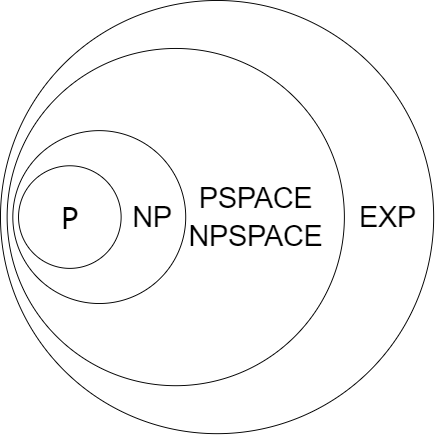
\includegraphics[scale = .3]{imm/Untitled Diagram.png}
\end{figure}


Abbiamo anche le classi $CO\_P$ e $CO\_NP$, ovvero le classi dei problemi complementari $P$ e $NP$. Si ha che, grazie al determinismo, cambiando semplicemente la risposta data in output, possiamo dire $CO\_P=P$\\
Quando si introduce il non determinismo le cose cambiano. La domanda iniziale era del tipo \textit{esiste almeno uno} quindi il completamento è \textit{non esiste nessuno}, quindi devo verificare tutti i casi, andando in un caso che nemmeno la NDTM riesce a risolvere, si finisce infatti nella classe $EXP$. \\ Quindi si ha che:
$P\subseteq CP\_NP\land P\subseteq NP$ non avendo un rapporto diretto e definito tra $NP$ e $CO\_NP$.